\documentclass[13pt, a4paper]{extreport}
\usepackage[utf8]{vietnam}  
\usepackage{type1cm}
\usepackage{listings}
\usepackage{fancybox}
\usepackage{fancyhdr}
\usepackage[left=3.40cm, right=2.00cm, top=2cm, bottom=2cm]{geometry}
\usepackage{graphicx}
\linespread{1.5}
\usepackage{mathtools}
\usepackage{mathptmx}
\usepackage{amsmath} %large sum
\usepackage{relsize} %large sum
\usepackage{etoolbox}
\usepackage{titlesec}
\usepackage{indentfirst}
\usepackage{enumitem}
\usepackage{float} %keep fixgure under text
\usepackage{tikz}

\usetikzlibrary{fit,positioning}

\fancypagestyle{plain}{
  \fancyhead{} 
  \renewcommand{\headrulewidth}{0pt}
  \fancyfoot{}
  \fancyfoot[LE,RO]{Trang \thepage} 
  \fancyfoot[RE,LO]{Sinh viên thực hiện: Lương Tiến Lâm – 20121957 – K57 – CNTT-TT2 2.04}
  \renewcommand{\footrulewidth}{0.1pt}
}
\renewcommand{\baselinestretch}{1.0}


\titleformat{\chapter}[block]
  {\normalfont\LARGE\bfseries}{\chaptertitlename\ \thechapter:}{0pt}{\Large}[{\vspace{0ex}\titlerule[2pt]}]

\titleformat{\section}
  {\normalfont\fontsize{14}{16.8}\bfseries}{\thesection}{1em}{}
\titleformat{\subsection}
  {\normalfont\fontsize{14}{16.8}\bfseries}{\thesubsection}{1em}{}

\titlespacing*{\chapter}{0pt}{0pt}{5pt}

\setlist{parsep=0pt,listparindent=\parindent}

\begin{document}
\thispagestyle{empty}
\thisfancypage{
\setlength{\fboxsep}{3pt}
\fbox}{}

\pagestyle{plain}
\begin{center}
{\fontsize{16}{19.2}\selectfont{TRƯỜNG ĐẠI HỌC BÁCH KHOA HÀ NỘI \\ VIỆN CÔNG NGHỆ THÔNG TIN - TRUYỀN THÔNG}} \\
\textbf{------------------------  *  ------------------------}\\
\vspace{1.3in}
\begin{center}
{\fontsize{32pt}{38.4}\selectfont {ĐỒ ÁN}}\\
\vspace{0.05in}
{\fontsize{38pt}{45.6}\selectfont \textbf{TỐT NGHIỆP ĐẠI HỌC}}\\
\vspace{0.12in}
{\fontfamily{phv} \fontsize{20pt}{24}\selectfont {NGÀNH CÔNG NGHỆ THÔNG TIN}}\\
\vspace{1.3in}
{\fontsize{22pt}{26.4}\selectfont {\textbf{XÂY DỰNG MÔ HÌNH HPC TRONG ỨNG DỤNG GÁN ĐA NHÃN ẢNH}}}
\end{center}


\vspace{0.45in}
\begin{flushleft}
{\hspace{1.8in}{\fontsize{14pt}{16.8}\selectfont {Sinh viên thực hiện:\hspace{0.12in} \textbf{Lương Tiến Lâm}}}}\\
{\hspace{1.8in}\hspace{1.215in}\fontsize{14pt}{16.8}\selectfont {Lớp: CNTT-TT 2.04 - K57}}\\
{\hspace{1.8in}{\fontsize{14pt}{16.8}\selectfont {Giáo viên hướng dẫn: TS \textbf{Nguyễn Thị Oanh}}}}\\
\end{flushleft}
\end{center}
\vspace{1.9in}
\begin{center}
{\fontsize{16pt}{1}\selectfont Hà Nội 5-2017 }\\
\end{center}

\newpage
\begin{center}
{\fontsize{16pt}{19.2}\selectfont \textbf{PHIẾU GIAO NHIỆM VỤ ĐỒ ÁN TỐT NGHIỆP}}
\end{center}	
\begin{enumerate}
  \fontsize{13pt}{15.6}\selectfont
  \item Thông tin về sinh viên \\
   Họ và tên sinh viên: LƯƠNG TIẾN LÂM \\
   Điện thoại liên lạc: 01245021194 \hspace{2cm} Email: lamluongbka@gmail.com \\
   Lớp:CNTT-TT2 2.04 \hspace{4.28cm} Hệ đào tạo: Đại học chính quy \\
   Đồ án tốt nghiệp được thực hiện tại: Bộ môn Khoa học máy tính, Viện Công nghệ thông tin và truyền thông, Đại học Bách Khoa Hà Nội.
  Thời gian làm ĐATN: Từ ngày 12/01/2017 đến 29/05/2017
  \item Mục đích nội dung của ĐATN \\
  \begin{itemize}
    \item Nghiên cứu mạng học sâu GGNet VGG
    \item Nghiên cứ thuật toán BING
    \item Áp dụng mạng học sâu trong bài toán gán đa nhãn ảnh
  \end{itemize}
  \item Các nhiệm vụ cụ thể của ĐATN \\
  \item Lời cam đoan của sinh viên:\\
   Tôi – Lương Tiến Lâm - cam kết ĐATN là công trình nghiên cứu của bản thân tôi dưới sự hướng dẫn của TS.Nguyễn Thị Oanh. \\
   Các kết quả nêu trong ĐATN là trung thực, không phải là sao chép toàn văn của bất kỳ công trình nào khác.
  \begin{flushleft}
    {\fontsize{13pt}{15.6pt}\selectfont {
      \hspace{3in}Hà Nội, ngày \hspace{0.5cm} tháng \hspace{0.5cm} năm 2017 \\
      \hspace{3.7in}Tác giả ĐATN \\
      \hspace{3.5in}\textit{(Ký và ghi rõ họ tên)}\\[1.5cm]}
    }
  \end{flushleft}
  \item Xác nhận của giáo viên hướng dẫn về mức độ hoàn thành của ĐATN và cho phép bảo vệ:
    \begin{flushleft}
	  {\fontsize{13pt}{15.6pt}\selectfont {
        \hspace{3in}Hà Nội, ngày \hspace{0.5cm} tháng \hspace{0.5cm} năm 2017 \\
        \hspace{3.5in}Giáo viên hướng dẫn \\
        \hspace{3.5in}\textit{(Ký và ghi rõ họ tên)}\\[1.5cm]
        }
      }
  	\end{flushleft}
\end{enumerate}

\newpage
\chapter*{\centerline{TÓM TẮT NỘI DUNG ĐỒ ÁN TỐT NGHIỆP}}
\fontsize{13}{15.6}\selectfont
\setlength{\parindent}{0.7cm}
Thời đại bùng nổ về công nghệ thông tin con người đang không những chỉ muốn các công cụ mình sử dụng phải thật thuận tiên, giảm thời gian thao tác mà nó còn phải thông minh, có thể biết được người dung muôns gì ngay cả khi chưa được ra lệnh. Quả thực trong thời gian qua, ngành Trí Tuệ Nhân Tạo nói chung và Học Máy nói riêng đang có bước phát triển đột phá không ngừng, nhờ sự phát triển đó mà các thiết bị mà con nguwoif sử dụng đang ngày càng tỏ ra thông minh vượt bậc thậm chí là vượt qua cả sự nhận thức của con người.\\
\indent Mạng học sâu là một nhánh của ngành khoa học máy tính kể trên và bài toán huấn luyện cho máy tính về một tri thức dựa trên một tập dữ liệu sẵn có không phải bài toán mới nhưng nó vẫn đang phát triển không ngừng và tương lai còn hứa hẹn ra những thành tựu lớn.\\
\indent Trong đồ án này tác giả tập trung vào bài toán gán đa nhãn ảnh mà cụ thể là gán nhãn cho bức ảnh chụp nhiều đồ ăn, đưa ra nhiều và đúng nhất có thể các món ăn có trong bức ảnh dựa vào Mạng học sâu và thuật toán nhận dạng các đối tượng trong ảnh.\\
\indent Nôi dung đồ án gồm các chương chính sau:

\newpage
\chapter*{\centerline{LỜI NÓI ĐẦU}}
\indent Nhận dạng nội dung hay khái quát hơn là gán nhãn cho ảnh là bài toán đã được quan tâm từ lâu và đã vượt qua phạm trù lý thuyết đơn thuần và tiến tới ứng dụng thực tế. có rất nhiều ứng dụng dựa trên detech và gán nhãn ảnh được các ông lớn sử dụng và rất thành công dù chỉ là opensorce nhưng cũng kiếm được các khoản lợi nhuận khổng lồ như tag ảnh của fb hay google draw của google
Nói về ẩm thực thì chúng ta đã biết độ phong phú và đa dạng của lĩnh vực này, có hàng ngàn các món ăn trên thế giớ trải dài từ bán cầu Tây sang Đông và ngay cả ở Việt Nam hệ thống ẩm thực khá phong phú nhwung không phải món ăn nào ta cũng biết. \\
\indent Việc gán nhãn cho các món ăn hiên đang rất được các nhà phát triển web. app quan tâm. và mạng xã hội ẩm thực hiện nay mới chỉ dừng ở mức độ   gán nhãn ảnh dựa trên nhãn mà người dùng gãn sẵn vào. việc up một bức ảnh lên mà người dùng không gán nhãn thì vẫn đang chưa thực hiện được. \\
\indent Ở trong bài toán này yêu cầu được đưa ra như sau: đưa một ảnh đầu vào chụp một hoặc nhiều món ăn. nhiệm vụ của máy tính phải phát hiện được nhiều món ăn nhất có thể và gán nhãn cho ảnh là tên các mon ăn mà nó phát hiên được.
Có rất nhiều mô hình, mạng học sâu có thê giải quyết được bài toán này nhưng trong khuôn khổ đồ án tác gỉa sử dụng mô hình mạng googlenet để làm mô hình tranning và detecting, thuật tón BING để khoanh vùng các món ăn trong ảnh.

\tableofcontents
\newpage

\newpage
\chapter{\centerline{MẠNG NEURAL NHÂN TẠO}}
\section{Cấu Trúc một NơRon}
Mạng nơron nhân tạo, Artificial Neural Network (ANN) là một mô hình xử lý dữ liệu mô phỏng theo hoạt động của bộ não sinh vật. Thành phần cơ bản cấu tạo nên một mạng nơron cũng như của não bộ đó chính là nơron. Ta xét mô hình:\\
\begin{figure}[H]
\centering
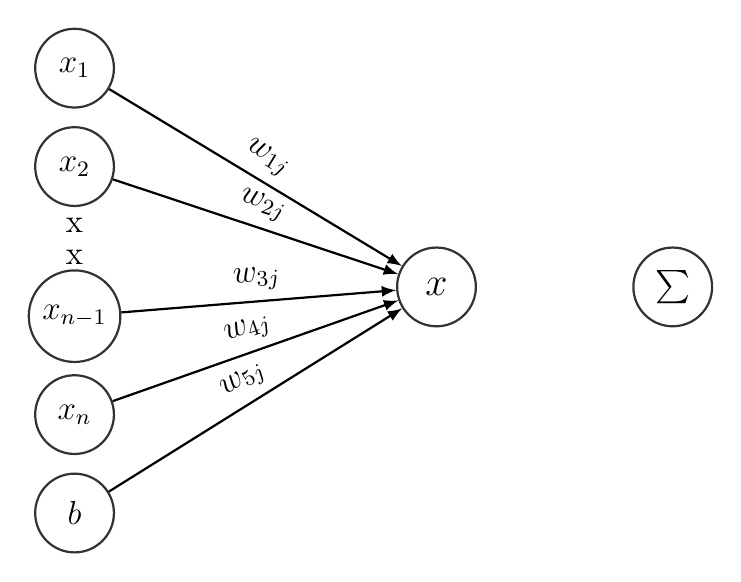
\begin{tikzpicture}
\tikzstyle{main}=[circle, minimum size = 10mm, thick, draw =black!80, node distance = 16mm]
\tikzstyle{connect}=[-latex, thick]
\tikzstyle{box}=[rectangle, draw=black!100]
  \node[main, fill = white!100] (sigma) [] {\Large $x$};
  \node(x1) [above left=0.2cm and 4cm of sigma] {\large x};
  \node(x2) [node distance=0.4cm, below of=x1] {\large x};
  \node[main] (x3) [node distance=0.75cm, above of=x1] {\large $x_2$};
  \node[main] (x4) [node distance=1.25cm, above of=x3] {\large $x_1$};
  \node[main] (x5) [node distance=0.75cm, below of=x2] {\large $x_{n-1}$};
  \node[main] (x6) [node distance=1.25cm, below of=x5] {\large $x_n$};
  \node[main] (x7) [node distance=1.25cm, below of=x6] {\large $b$};
  \node[main] (x8) [node distance=3cm, right of=sigma] {\large $\sum$};
%  \node[main] (z) [left=of alpha,label=below:z] {};
%  \node[main] (beta) [left=of alpha,label=below:$\beta$] { };
%  \node[main, fill = black!10] (w) [left=of alpha,label=below:w] {};
  
  \path [every node/.style={sloped,anchor=south,auto=false}]
  		(x3) edge [connect] node {\large $w_{2j}$}(sigma)
  		(x4) edge [connect] node {\large $w_{1j}$}(sigma)
  		(x5) edge [connect] node {\large $w_{3j}$}(sigma)
  		(x6) edge [connect] node {\large $w_{4j}$}(sigma)
  		(x7) edge [connect] node {\large $w_{5j}$}(sigma);
%        (theta) edge [connect] (z)
%		(z) edge [connect] (w)
%		(beta) edge [connect] (w);
\end{tikzpicture}
\end{figure}

Theo sơ đồ trên ta thấy rằng một nơron có các thành phần cơ bản sau:
\begin{itemize}
\item Input: Các tín hiệu đầu vào, thường được đưa vào dưới dạng vector n chiều:\\
	\centerline {$X = \{x_0, x_1, ..., x_m\}$}
\item Tập liên kết (Connections): thể hiện sự liên kết của tín hiệu với nơron.
\item Trọng số liên kết (Connection weight): thể hiện mức độ của liên kết đối với nơron, mỗi một vector tín hiệu đầu vào sẽ có một vector trọng số liên kết tương ứng:\\
	\centerline {$W = \{w_0, w_1, ..., w_m\}$}
\item Hàm tổng (Summation Function): Một hàm tuyến tính, tính tổng các tích giữa Input với trọng số liên kết tương ứng:\\
	\centerline {$Net = w_0 + w_1x_1 + w_2x_2 + ... + w_mx_m = w_0 + \sum\limits_{i=1}^m w_ix_i$}
\item Hàm truyền: Nhận đầu vào là kết quả của hàm tổng, giới hạn ngưỡng của nơron, tính toán đầu ra của nơron. ta có một số loại hàm truyền:
	\begin{itemize}
		\item Hàm ngưỡng (threshold function):
		  \begin{center}
			$Output = \begin{dcases} 1, & \text{if } Net \geq \theta\\ 0, & \text{otherwise} \end{dcases}$
		  \end{center}	
		Với $\theta$ là giá trị ngưỡng. Hàm có đặc điểm là không liên tục và không có đạo hàm. Thường được sử dụng trong các bài toán chỉ có 2 kết quả (có - không, đúng - sai ...).
		\item Hàm logic ngưỡng (threshold Logic function):
     	  \begin{center}
			$Output = 
				\begin{dcases} 
					0, & \text{if } Net < -\theta \\
					\alpha(Net + \theta), & \text{if } -\theta \leq Net \leq \frac{1}{\alpha}-\theta\\
					1, & \text{if } Net > \frac{1}{\alpha}-\theta
				\end{dcases}$
		  \end{center}
		  Còn được gọi là  hàm tuyến tính bão hòa, là sự kết hợp của hàm tuyến tính và giới hạn chặ. Đặc điểm là liên tục nhưng không có đạo hàm.
		\item Hàm Sigmoid:
		  \begin{center}
			$Output = \dfrac{1}{1 + e^{-\alpha(Net + \theta)}}$
		  \end{center}
		  Là hàm liên tục và có đạo hàm, cho giá trị đầu ra trong khoảng (0, 1) và được dùng phổ biến nhất. Đạo hàm của hàm Sigmoid chính là hàm Sigmoid. Được sử dụng trong các bài toán dự đoán nhiều kết quả.
		\item Hàm Hyperbolic tangent:
		   \begin{center}
			$Output = \dfrac{1 - e^{-\alpha(Net + \theta)}}{1 + e^{-\alpha(Net + \theta)}}
					= \dfrac{2}{1 + e^{-\alpha(Net + \theta)}} - 1$
		  \end{center}  
		 Giống hàm sigmoid, liên tục và có đạo hàm, cho giá trị đầu ra trong khoảng (-1, 1).  
	\end{itemize}
	\item Độ lệch (bias): $w_0$ là một hệ số để điều chỉnh kết quả đầu ra của hàm tổng theo ý muốn mà không phải thay đổi giá trị của trọng số liên kết (sẽ đề cập ở bên dưới), tránh gấy ảnh hưởng tới kết quả tính của nơron khác. Ví dụ muốn thay đổi giá trị kết quả đầu ra thay vì phải thay đổi giá trị bộ trọng số, ta có thể điểu chỉnh giá trị độ lệch bias. Mặt khác, họ các hàm $Net = w_0 + \sum\limits_{i=1}^m w_ix_i$ có thể chia các tập ví dụ thành nhiều lớp, họ các hàm $Net = \sum\limits_{i=1}^m w_ix_i$ do đi qua gốc $O(0; 0)$ trong nhiều trường hợp không thể phân tách được các ví dụ.
\end{itemize}

\indent Như vậy, từ input đầu vào X, thông qua các hàm xử lý cùng với các trọng số liên kết, một nơron cho ra một kết quả đầu ra. Kết quả đầu ra này có thể là kết quả cuối hoặc là đầu vào của một nơ ron khác.
\section{Cấu Trúc một mạng Nơron}
\indent Mạng nơron nhân tạo được cấu trúc theo các tầng, mỗi tầng chứa một nhóm các nơron: (Ảnh minh họa)
\begin{itemize}
\item Tầng đầu vào(Input layer).
\item Tầng đầu ra(Ouput layer).
\item Tần ẩn (Hiden Layer) có hoặc không cần tầng này, là tầng nằm giữa tầng đầu vào và đầu ra, các nơron ở tầng này không trực tiếp tương tác với môi trường ngoài mà đầu vào của nơ ron thường là kết quả đầu ra của nơ ron khác.
\end{itemize}

\indent Cách thức kết nối của các nơ ron trong mạng xác định kiến trúc (topology) của mạng. Một mang nơ ron được gọi là đầy đủ nếu như mọi đầu ra của nơ ron từ một tầng liên kết với mọi nơron ở tầng kế tiếp, còn ngược lại, đầu ra của một số nơ ron chỉ liên kết với một sô nơ ron khác được gọi là kết nỗi cục bộ. Có nhiều kiểu mạng nơ ron nhưng ta xet các loại chính sau:
\begin{itemize}
\item Mạng nơ ron lan truyền tiến: kết quả của một nơ ron là đầu vào của nơ ron tâng kế tiếp, đầu ra của một tầng bất kì không ảnh hưởng tới tầng đó, các tín hiệu di chuyển theo đường thằng, không có kết nối ngược lại từ các tầng phía sau về các tầng ở phía trước.
\item Mạng nơ ron lan truyền ngược (): kiểu kiến trúc có sự kết nối từ nơ ron ở tầng đầu ra về nơ ron ở tầng đầu vào, kiểu kiến trúc này lưu lại trạng thái trước đó vì thế kêt quả của trạng thái tiếp theo không chỉ phụ thuộc vào các tín hiệu đầu vào mà còn phụ thuộc vào trạng thái trước đó của mạng.
\end{itemize}
\section{Huấn luyện mạng nơ ron nhân tạo}
Xét một tập dữ liệu X được dùng để huấn luyện mạng nơ ron, tập Y là tập kết quả của tập dữ liệu X. Ta gọi tập X ở trên là tập học (traning set) còn tập Y là các nhãn tương ứng. Nhiệm vụ của việc huấn luyện mạng nơ ron là điều chỉnh các trọng số liên kết trong tập W của nó sao cho đối với mọi đầu vào $x_i$ từ tập X mạng cho ra một kết quả $y_i$ tương ứng ở tập Y.
\subsection{Các Phương Pháp học}
\begin{itemize}
	\item Học không giám sát:\\
	\indent Là kiểu học mà tập X chưa biết trước các nhãn tương ứng của nó. Nhiệm vụ của mạng nơ ron lúc này là tìm cách chia tập dữ liệu ban đầu thành các nhóm, mỗi nhóm chứa các đặc trưng giống nhau.\\
	\indent Học không giám sát được sử dụng khi chưa biết số lượng các lớp cần được phân loại, việc chia ra thành các lớp phụ thuộc vào tiêu chuẩn đánh giá độ tương tự giữa các dữ liệu.
	\item Học có giám sát:\\
	\indent Là kiểu học mà tập học X đã biết trước số lượng nhãn cần phân cụm và nhãn tương ứng của từng dữ liệu. Nhiệm vụ của mạng nơ ron lúc này là lưu lọc ra các đặc trưng của từng dữ liệu trong X và gán tương ứng từng đặc trưng của dữ liệu đó với nhãn trong Y. Khi có một dữ liệu mới đến không nằm trong tập dữ liệu trong X, mạng nơron phải trích xuất được các đặc trưng của dữ liệu mới đó rồi so sánh để lấy ra được nhãn cho dữ liệu.\\
	\indent Học có giám sát được sử dụng khi mà ta có tập học X đủ lớn để học được nhiều nhất có thể đặc trưng của từng nhãn.
\end{itemize}
\subsection{Huấn luyện mạng nơron theo phương pháp học không giám sát}
\indent Xét tập học X và tập nhãn Y, ta có ánh xạ tương ứng X->Y, $x_i = {x_0, x_1, ..., x_m}$ là một dữ liệu (vector) thuộc X có nhãn tương ứng $y_i$.
\begin{itemize}
	\item Dựng mô hình mạng nơron 
\end{itemize}

\chapter{\centerline{CONVOLUTION NEURAL NETWORK}}
\section{Khái niệm}
\indent Mô hình mạng nơron nhân tạo ra đời đã được áp dụng nhiều trong các bài toán nhận. Tuy nhiên mạng nơron nhân tạo thông thường không phát huy tốt hiệu quả khi xử lý các dữ liệu lớn như hình ảnh, video... Một tấm ảnh xám có kích thước 32x32 pixel sẽ cho ra vector đặc trưng 1024 chiều, còn đối với ảnh màu có cùng kích thước sẽ là 3072 chiều. Vector có số chiều như vậy khá là lớn đối với mạng nơron thông thường, để xử lý được mạng nơron cũng phải có 3072 bộ trọng số tương  giữa tầng Input và nơron tầng ẩn. Như thế đối với mạng có nhiều node hoặc có nhiều tầng ẩn thì số lượng trọng số sẽ càng bị nhân rộng thêm. Với ảnh có kích thước bình thường (vẫn lớn hơn ảnh 32x32 rất nhiều) thì việc tính toán trên mạng sẽ gặp rất nhiều khó khăn.
\indent Mặt khác để ý rằng việc liên kết mọi điểm ảnh vào một node trong mạng là dư thừa bởi vì đối với dữ liệu ảnh thì các điểm ảnh ở gần nhau mới có sự phụ thuộc (điểm tương đồng) với nhau, các điểm ảnh càng xa nhau thì càng ít phụ thuộc vào nhau. Do đặc trưng trên nên người ta nghĩ ra việc thay vì kết nối toàn bộ các điểm ảnh với một node thì chỉ có một phần cục bộ trong ảnh được kết nối tới node ở lớp tiếp theo, gọi là kết nối cục bộ (Local Connectivity). Hệ thống dựa trên các lớp của mô hình sẽ học ra được các đặc trưng của ảnh để việc phân lớp được tiến hành hiệu quả.
  \begin{figure}[H]
  	\centering
    \includegraphics[width=15cm]{Convolution}
    \caption{\large Minh họa một mạng CNN}
  \end{figure}
\indent Mạng nơron nhân chập hay mạng convolution neural network hay gọi tắt là CNN là một loại hình của mạng nơron lan truyền tiến, nó gồm có các tầng chính sau: Convolutional, Pooling, Revolution Liner Unit (RELU) và Fully Connected. Tùy từng mục đích của bài toán mà người ta dựng lên các mô hinh với số tầng và thứ tự giữa các tầng là khác nhau.

\section{Các tầng của CNN}
\subsection{Convolution}
\indent Đây là tầng đặc trưng nhất của CNN, thay vì kết nối toàn bộ các điểm ảnh, mô hình sẽ tạo ra các bộ lọc (hay còn gọi là cửa sổ trượt) có kích thước nhỏ hơn so với ảnh, thường là 3x3 hoặc là 5x5 áp vào vùng trong góc ảnh rồi tiến hành phép nhân chập (convolution). Bộ lọc sẽ được trượt dọc theo biên rồi trượt qua toàn bộ các vùng của ảnh. Mỗi lần trượt, bộ lọc sẽ dịch chuyển một bước trượt (stride). \\
\indent Công thức tích chập giữa hàm ảnh f(x, y) và bộ lọc k(x, y) (kích thước mxn):
\begin{center}
$k(x, y) * f(x, y) = \mathlarger{\sum\limits_{u=-\frac{m}{2}}^{\frac{m}{2}}\sum\limits_{u=-\frac{n}{2}}^{\frac{n}{2}}}k(u, v)f(x-u, y-v) $
\end{center}

\begin{figure}[H]
  \centering
    \includegraphics[width=15cm]{convolution1}
   \caption{\large Nhân chập ảnh với bộ lọc.}
\end{figure}

\indent Như vậy với một bức ảnh 32x32 và một fitter 3x3 ta sẽ có một ảnh mới kích thước 32x32 (việc padding bộ lọc đã đảm bảo cả điểm ảnh ở ngoài biên bức ảnh đều được thực hiện nhân chập) là kết quả của việc nhân chập ảnh gốc với bộ lọc. Số lượng ảnh trả ra cho các lớp tiếp theo bằng với số lượng filter nhân chập với ảnh. Các filter ban đầu được khởi tạo ngẫu nhiên và sẽ được điều chỉnh trong quá trình học. Như vậy thực chất của việc học trong mạng CNN là tìm ra các filter thích hợp nhất để lọc ra các đặc trưng của ảnh.
\subsection{Rectified Linear Unit - RELU}
\indent Được sử dụng ngay sau tầng Convolutionm dùng hàm kích hoạt $f(x) = max(0, x)$ có nhiệm vụ chuyển toàn bộ giá trị âm trong kết quả của việc nhân chập thành giá trị 0. Hàm này tạo nên tính phi tuyến của mô hình. Có thể sử dụng các hàm phi tuyến thông dụng như sigmoid, tanh nhưng hàm max được đánh giá là dễ cài đặt và hiệu quả hơn.
\begin{figure}[H]
  \centering
    \includegraphics[width=12cm]{relu}
   \caption{\large Rectified Linear Unit.}
\end{figure}
\subsection{Pooling}
\indent Tầng này sử dụng một cửa sổ trượt quét qua toàn bộ ảnh dữ liệu, mỗi lần trượt theo một bước trượt (stride) cho trước. Khác với lớp Convolutional, lớp Pooling không tính tích chập mà tiến hành lấy mẫu (subsampling). Khi cửa sổ trượt trên ảnh, chỉ có một giá trị được xem là giá trị đại diện cho thông tin ảnh tại vùng đó (giá trị mẫu) được giữ lại. Các phương thức lấy phổ biến trong lớp Pooling là MaxPooling ( lấy giá trị lớn nhất), MinPooling (lấy giá trị nhỏ nhất) và AveragePooling (lấy giá trị trung bình).
\begin{figure}[H]
  \centering
    \includegraphics[width=12cm]{pooling}
   \caption{\large Max Pooling.}
\end{figure}

\indent Xét một ảnh có kích thước 32x32 và lớp Pooling sử dụng filter có kích thước 2x2 với bước trượt stride = 2, phương pháp sử dụng là MaxPooling. Filter sẽ lần lượt duyệt qua ảnh, với mỗi lần duyệt chỉ có giá trị lớn nhất trong 4 giá trị nằm trong vùng cửa sổ 2x2 của filter được giữ lại và đưa ra đầu ra. Như vậy sau khi qua lớp Pooling, ảnh sẽ giảm kích thước xuống còn 16x16 (kích thước mỗi chiều giảm 2 lần).

\subsection{Fully Connected(FC)}
\indent Tầng này tương tự với lớp trong mạng nơ-ron truyền thẳng, các giá trị ảnh được liên kết đầy đủ vào node trong lớp tiếp theo. Sau khi ảnh được xử lý và rút trích đặc trưng từ các lớp trước đó, dữ liệu ảnh sẽ không còn quá lớn so với mô hình truyền thẳng nên ta có thể sử dụng mô hình truyền thẳng để tiến hành nhận dạng. Tóm lại, lớp fully-connected đóng vai trò như một mô hình phân lớp và tiến hành dựa trên dữ liệu đã được xử lý ở các lớp trước đó.
\begin{figure}[H]
  \centering
    \includegraphics[width=11cm]{fully}
   \caption{\large Mạng CNN đầy đủ các tầng}
\end{figure}
\section{Huấn luyện mạng CNN}
\indent Một mạng nơ-ron tích chập được hình thành bằng cách ghép các lớp nêu trên lại với nhau. Mô hình bắt đầu với lớp Convolutional. Tầng RELU thường luôn được cài đặc ngay sau tầng Convolutional hoặc thậm chí kết hợp cả hai tầng này thành một tầng. Các tầng tiếp theo có thể là Convolutional hay Pooling tùy theo kiến trúc mà ta muốn xây dựng. Cuối cùng sẽ là lớp fully-connected để tiến hành phân lớp.\\
\indent Để xem mô hình này hoạt động như thế nào ta có thể xét một kiến trúc sau đây:
\begin{center}
\textit{Conv1 (with RELU) – Pooling – Conv2 (with RELU) – Pooling – FC – FC}
\end{center}
\indent Lấy một hình ảnh cần nhận dạng có kích thước 32x32 như sau (lấy từ bộ dữ liệu cifar-10):
\begin{figure}[H]
  \centering
    \includegraphics[width=11cm]{origin_cifa}
   \caption{\large một ảnh đầu vào}
\end{figure}
\indent Hình ảnh sẽ được đưa vào tầng Conv1 (Convolutional kết hợp RELU) gồm 32 filter có kích thước 3x3, mỗi filter sẽ được dùng để tính tích chập với ảnh và cho ra một ảnh kết quả tương ứng. Với 32 filter ta sẽ có 32 ảnh kết quả như sau:
\begin{figure}[H]
  \centering
    \includegraphics[width=13cm]{conv}
   \caption{\large một ảnh đầu vào}
\end{figure}

\indent Mỗi ảnh trên đều có kích thước tương ứng là 32x32. Sau đó, cả 32 ảnh này đều được cho qua lớp Pooling và kết quả trả ra sẽ là 32 ảnh có kích thước 16x16.\\
\indent Tiếp tục dữ liệu sẽ đi vào lớp Conv2. Tương tự như Conv1, ảnh sẽ được tính tích chập với filter và trả ra kết quả. Lớp Pooling tiếp theo sẽ tiếp tục giảm kích thước của ảnh xuống còn 8x8. Với kích thước đủ nhỏ như vậy, lớp Fully-connected tiếp theo sẽ xử lý và đưa ra kết quả phân lớp hay kết quả nhận dạng.\\
\indent Tương tự như mạng nơ-ron truyền thẳng, mạng nơ-ron tích chập cũng là một mô hình học cho nên khởi tạo ban đầu cho các trọng số trong mạng là ngẫu nhiên và sẽ được điều chỉnh thông qua quá trình học. Thuật toán học cho mạng nơ-ron tích chập cũng tương tự như mạng nơ-ron truyền thẳng là thuật toán lan truyền ngược sử dụng gradient descent; chỉ khác nhau ở chỗ mạng tích chập không liên kết đầy đủ nên độ lỗi ở mỗi lớp chỉ tính dựa vào một phần các node trong lớp tiếp theo chứ không phải toàn bộ.
\chapter{\centerline{BINARIZED NORMED GRADIENTS}}
\indent 
\end{document}















